\documentclass[11pt,a4paper]{article}

% --- PAQUETES DE IDIOMA Y CODIFICACIÓN ---
\usepackage[utf8]{inputenc}
\usepackage[T1]{fontenc}
\usepackage[spanish,es-tabla,es-nodecimaldot,es-noshorthands]{babel}

% --- MATEMÁTICAS Y SÍMBOLOS ---
\usepackage{amsmath,amssymb,amsfonts}
\usepackage{mathtools}

% --- FORMATO Y DISEÑO DE PÁGINA ---
\usepackage[top=2.5cm, bottom=2.5cm, left=2.5cm, right=2.5cm]{geometry}
\usepackage{fancyhdr}
\usepackage{booktabs}
\usepackage{array}
\usepackage{enumitem}
\usepackage{titlesec}
\usepackage{graphicx}

% --- COLORES Y CÓDIGO ---
\usepackage[table]{xcolor}
\definecolor{pujblue}{RGB}{0, 51, 102}
\definecolor{darkblue}{RGB}{16, 44, 87}
\definecolor{codebg}{RGB}{248, 249, 250}
\definecolor{darkgray}{RGB}{60, 60, 60}

\usepackage{listings}
\usepackage[colorlinks=true, linkcolor=pujblue, citecolor=pujblue, urlcolor=pujblue]{hyperref}

% --- CONFIGURACIÓN DE LISTINGS ---
\lstset{
    language=Python,
    backgroundcolor=\color{codebg},
    basicstyle=\ttfamily\footnotesize,
    keywordstyle=\color{pujblue}\bfseries,
    commentstyle=\color{gray}\itshape,
    stringstyle=\color{teal},
    breaklines=true,
    frame=single,
    rulecolor=\color{black!20},
    numbers=left,
    numberstyle=\tiny\color{gray},
    numbersep=8pt,
    tabsize=4,
    showstringspaces=false,
    literate=
      {á}{{\'a}}1 {é}{{\'e}}1 {í}{{\'i}}1 {ó}{{\'o}}1 {ú}{{\'u}}1
      {Á}{{\'A}}1 {É}{{\'E}}1 {Í}{{\'I}}1 {Ó}{{\'O}}1 {Ú}{{\'U}}1
      {ñ}{{\~n}}1 {Ñ}{{\~N}}1 {ü}{{\"u}}1 {Ü}{{\"U}}1
      {¿}{{?`}}1 {¡}{{!`}}1
}

% --- ENCABEZADOS Y PIES DE PÁGINA ---
\pagestyle{fancy}
\fancyhf{}
\fancyhead[L]{\small\color{darkgray}\textit{Computación Científica}}
\fancyhead[R]{\small\color{darkgray}\textit{Taller de Integración Numérica}}
\fancyfoot[C]{\thepage}
\renewcommand{\headrulewidth}{0.4pt}
\renewcommand{\footrulewidth}{0.4pt}

\titleformat{\section}{\Large\bfseries\color{pujblue}}{\thesection}{1em}{}[\titlerule]
\titleformat{\subsection}{\large\bfseries\color{darkblue}}{\thesubsection}{1em}{}
\titleformat{\subsubsection}{\normalsize\bfseries\color{darkblue}}{\thesubsubsection}{1em}{}

% ==============================================================================
% INICIO DEL DOCUMENTO
% ==============================================================================
\begin{document}

\begin{center}
    {\LARGE\bfseries\color{pujblue} Taller de Integración Numérica}\\[0.3cm]
    {\large Computación Científica --- Pontificia Universidad Javeriana Cali}\\[0.1cm]
    {\normalsize Profesor: Juan Fernando Paz}\\[0.1cm]
    {\normalsize Estudiante: Miguel Angel Padilla Rosero}
\end{center}
\vspace{0.3cm}

% ==============================================================================
% SECCIÓN 1: ALGORITMOS BASE EN PYTHON
% ==============================================================================
\section{Implementación de los Algoritmos Base en Python}

La integración numérica (o cuadratura numérica) aproxima la integral definida de una función $f:[a,b]\to\mathbb{R}$ evaluando combinaciones lineales de valores funcionales en nodos seleccionados. Para el desarrollo del taller se implementaron los métodos clásicos sobre particiones de $n$ subintervalos de paso $h = \frac{b-a}{n}$ y nodos $x_i = a + i h$ ($i=0,\dots,n$):

\begin{itemize}[leftmargin=*]
    \item \textbf{Suma de Riemann por la izquierda ($R_L$):} Aproxima el área en cada subintervalo mediante la altura del extremo izquierdo:
    \begin{equation}
        R_L(n) = h \sum_{i=0}^{n-1} f(x_i), \qquad \text{con error } E_{R_L} = O(h) = O(n^{-1}).
    \end{equation}
    \item \textbf{Suma de Riemann por la derecha ($R_R$):} Emplea la altura del extremo derecho:
    \begin{equation}
        R_R(n) = h \sum_{i=1}^{n} f(x_i), \qquad \text{con error } E_{R_R} = O(h) = O(n^{-1}).
    \end{equation}
    \item \textbf{Regla del Punto Medio compuesta ($M$):} Evalúa la función en los centros $m_i = x_i + \frac{h}{2}$:
    \begin{equation}
        M(n) = h \sum_{i=0}^{n-1} f\left(a + \left(i + \frac{1}{2}\right)h\right), \qquad E_M = \frac{(b-a)h^2}{24} f''(\eta) = O(n^{-2}).
    \end{equation}
    \item \textbf{Regla del Trapecio compuesta ($T$):} Interpola linealmente la función entre nodos consecutivos:
    \begin{equation}
        T(n) = \frac{h}{2} \left[ f(x_0) + 2 \sum_{i=1}^{n-1} f(x_i) + f(x_n) \right], \qquad E_T = -\frac{(b-a)h^2}{12} f''(\xi) = O(n^{-2}).
    \end{equation}
    \item \textbf{Regla de Simpson 1/3 compuesta ($S$):} Emplea interpolación cuadrática por pares de subintervalos ($n$ par):
    \begin{equation}
        S(n) = \frac{h}{3} \left[ f(x_0) + 4 \sum_{i=1,3,\dots}^{n-1} f(x_i) + 2 \sum_{i=2,4,\dots}^{n-2} f(x_i) + f(x_n) \right], \qquad E_S = -\frac{(b-a)h^4}{180} f^{(4)}(\zeta) = O(n^{-4}).
    \end{equation}
\end{itemize}

A continuación se presenta el código modular implementado en Python:

\begin{lstlisting}
import numpy as np

def riemann_izquierda(f, a, b, n):
    h = (b - a) / n
    x = a + np.arange(n) * h
    return h * np.sum(f(x))

def riemann_derecha(f, a, b, n):
    h = (b - a) / n
    x = a + np.arange(1, n + 1) * h
    return h * np.sum(f(x))

def punto_medio(f, a, b, n):
    h = (b - a) / n
    x_mid = a + (np.arange(n) + 0.5) * h
    return h * np.sum(f(x_mid))

def trapecio(f, a, b, n):
    h = (b - a) / n
    x = np.linspace(a, b, n + 1)
    y = f(x)
    return h * (0.5 * y[0] + np.sum(y[1:-1]) + 0.5 * y[-1])

def simpson_13(f, a, b, n):
    if n % 2 != 0:
        raise ValueError("n debe ser par para la regla de Simpson 1/3.")
    h = (b - a) / n
    x = np.linspace(a, b, n + 1)
    y = f(x)
    return (h / 3.0) * (y[0] + 4.0 * np.sum(y[1:-1:2]) + 2.0 * np.sum(y[2:-1:2]) + y[-1])
\end{lstlisting}

% ==============================================================================
% EJERCICIO 1
% ==============================================================================
\section{Ejercicio 1: Función polinómica}

Considere la integral definida:
\begin{equation}
    I = \int_0^3 (x^2 + 2x + 1)\, dx.
\end{equation}

\subsection{1. Cálculo del valor exacto de la integral}
La función integrando $f(x) = x^2 + 2x + 1 = (x+1)^2$ es continua y derivable en todo $\mathbb{R}$. Integrando término a término mediante el Teorema Fundamental del Cálculo:
\begin{align}
    F(x) &= \int (x^2 + 2x + 1)\, dx = \frac{x^3}{3} + x^2 + x, \\
    I &= F(3) - F(0) = \left( \frac{3^3}{3} + 3^2 + 3 \right) - (0) = \left( 9 + 9 + 3 \right) = \mathbf{21}.
\end{align}
Alternativamente, haciendo la sustitución simple $u = x+1$, $du = dx$:
\begin{equation}
    I = \int_1^4 u^2\, du = \left[ \frac{u^3}{3} \right]_1^4 = \frac{64 - 1}{3} = \frac{63}{3} = \mathbf{21}.
\end{equation}
El valor exacto de la integral es exactamente $I = 21$.

\subsection{2--4. Implementación de los métodos numéricos}
Se programaron las funciones \texttt{riemann\_izquierda}, \texttt{riemann\_derecha}, \texttt{punto\_medio} y \texttt{trapecio} presentadas en la Sección 1, evaluando sobre el intervalo $[a, b] = [0, 3]$.

\subsection{5. Comparación de errores para diferentes valores de $n$}
Se evaluaron los métodos para particiones diádicas con $n \in \{2, 4, 8, 16, 32, 64, 128, 256, 512, 1024\}$. En la Tabla~\ref{tab:ejercicio1_errores} se presentan los valores aproximados y el error absoluto $|I - I_n|$.

\begin{table}[h!]
\centering
\caption{Comparación de aproximaciones y errores absolutos para $I = \int_0^3 (x^2 + 2x + 1)\, dx = 21$.}
\label{tab:ejercicio1_errores}
\footnotesize
\begin{tabular}{rcccccccc}
\toprule
$n$ & $R_L(n)$ & Error $R_L$ & $R_R(n)$ & Error $R_R$ & $M(n)$ & Error $M$ & $T(n)$ & Error $T$ \\
\midrule
2   & $10.875000$ & $1.0125\times 10^{1}$ & $33.375000$ & $1.2375\times 10^{1}$ & $20.437500$ & $5.6250\times 10^{-1}$ & $22.125000$ & $1.1250\times 10^{0}$ \\
4   & $15.656250$ & $5.3438\times 10^{0}$ & $26.906250$ & $5.9062\times 10^{0}$ & $20.859375$ & $1.4062\times 10^{-1}$ & $21.281250$ & $2.8125\times 10^{-1}$ \\
8   & $18.257812$ & $2.7422\times 10^{0}$ & $23.882812$ & $2.8828\times 10^{0}$ & $20.964844$ & $3.5156\times 10^{-2}$ & $21.070312$ & $7.0312\times 10^{-2}$ \\
16  & $19.611328$ & $1.3887\times 10^{0}$ & $22.423828$ & $1.4238\times 10^{0}$ & $20.991211$ & $8.7891\times 10^{-3}$ & $21.017578$ & $1.7578\times 10^{-2}$ \\
32  & $20.301270$ & $6.9873\times 10^{-1}$ & $21.707520$ & $7.0752\times 10^{-1}$ & $20.997803$ & $2.1973\times 10^{-3}$ & $21.004395$ & $4.3945\times 10^{-3}$ \\
64  & $20.649536$ & $3.5046\times 10^{-1}$ & $21.352661$ & $3.5266\times 10^{-1}$ & $20.999451$ & $5.4932\times 10^{-4}$ & $21.001099$ & $1.0986\times 10^{-3}$ \\
128 & $20.824493$ & $1.7551\times 10^{-1}$ & $21.176056$ & $1.7606\times 10^{-1}$ & $20.999863$ & $1.3733\times 10^{-4}$ & $21.000275$ & $2.7466\times 10^{-4}$ \\
256 & $20.912178$ & $8.7822\times 10^{-2}$ & $21.087959$ & $8.7959\times 10^{-2}$ & $20.999966$ & $3.4332\times 10^{-5}$ & $21.000069$ & $6.8665\times 10^{-5}$ \\
512 & $20.956072$ & $4.3928\times 10^{-2}$ & $21.043962$ & $4.3962\times 10^{-2}$ & $20.999991$ & $8.5831\times 10^{-6}$ & $21.000017$ & $1.7166\times 10^{-5}$ \\
1024& $20.978032$ & $2.1968\times 10^{-2}$ & $21.021977$ & $2.1977\times 10^{-2}$ & $20.999998$ & $2.1458\times 10^{-6}$ & $21.000004$ & $4.2915\times 10^{-6}$ \\
\bottomrule
\end{tabular}
\end{table}

\paragraph{Análisis teórico de las razones de error:}
Calculando las derivadas de $f(x)$:
\begin{equation}
    f'(x) = 2x + 2, \qquad f''(x) = 2 \quad (\text{constante}), \qquad f'''(x) = 0.
\end{equation}
Como la segunda derivada $f''(x) = 2$ es una constante idéntica en todo el intervalo $[0, 3]$, el residuo de Taylor de orden 2 se vuelve exacto (no existen derivadas superiores):
\begin{align}
    E_T(n) &= -\frac{(b-a)^3}{12 n^2} f''(\xi) = -\frac{3^3}{12 n^2} (2) = -\frac{54}{12 n^2} = -\frac{4.5}{n^2}, \\
    E_M(n) &= \frac{(b-a)^3}{24 n^2} f''(\eta) = \frac{3^3}{24 n^2} (2) = \frac{54}{24 n^2} = \frac{2.25}{n^2}.
\end{align}
Esto conduce a dos conclusiones matemáticas de notable elegancia:
\begin{enumerate}
    \item Para cualquier $n$, el error absoluto del trapecio es \textbf{exactamente el doble} del error absoluto del punto medio:
    \begin{equation}
        |E_T(n)| = 2 \cdot |E_M(n)| = \frac{4.5}{n^2}.
    \end{equation}
    \item Dado que $f''(x) > 0$ (función estrictamente convexa), el trapecio siempre aproxima por exceso ($T > 21$) y el punto medio siempre aproxima por defecto ($M < 21$).
    \item Los métodos de Riemann por izquierda y derecha convergen con orden lineal $O(n^{-1})$, requiriendo aproximadamente 1000 subintervalos para alcanzar el error que el trapecio o el punto medio obtienen con apenas $n \approx 16$.
\end{enumerate}

En la Figura~\ref{fig:ejercicio1} se ilustra la interpretación geométrica de los trapecios superpuestos sobre el integrando y el gráfico log-log confirmando las pendientes asintóticas teóricas $-1$ y $-2$.

\begin{figure}[h!]
    \centering
    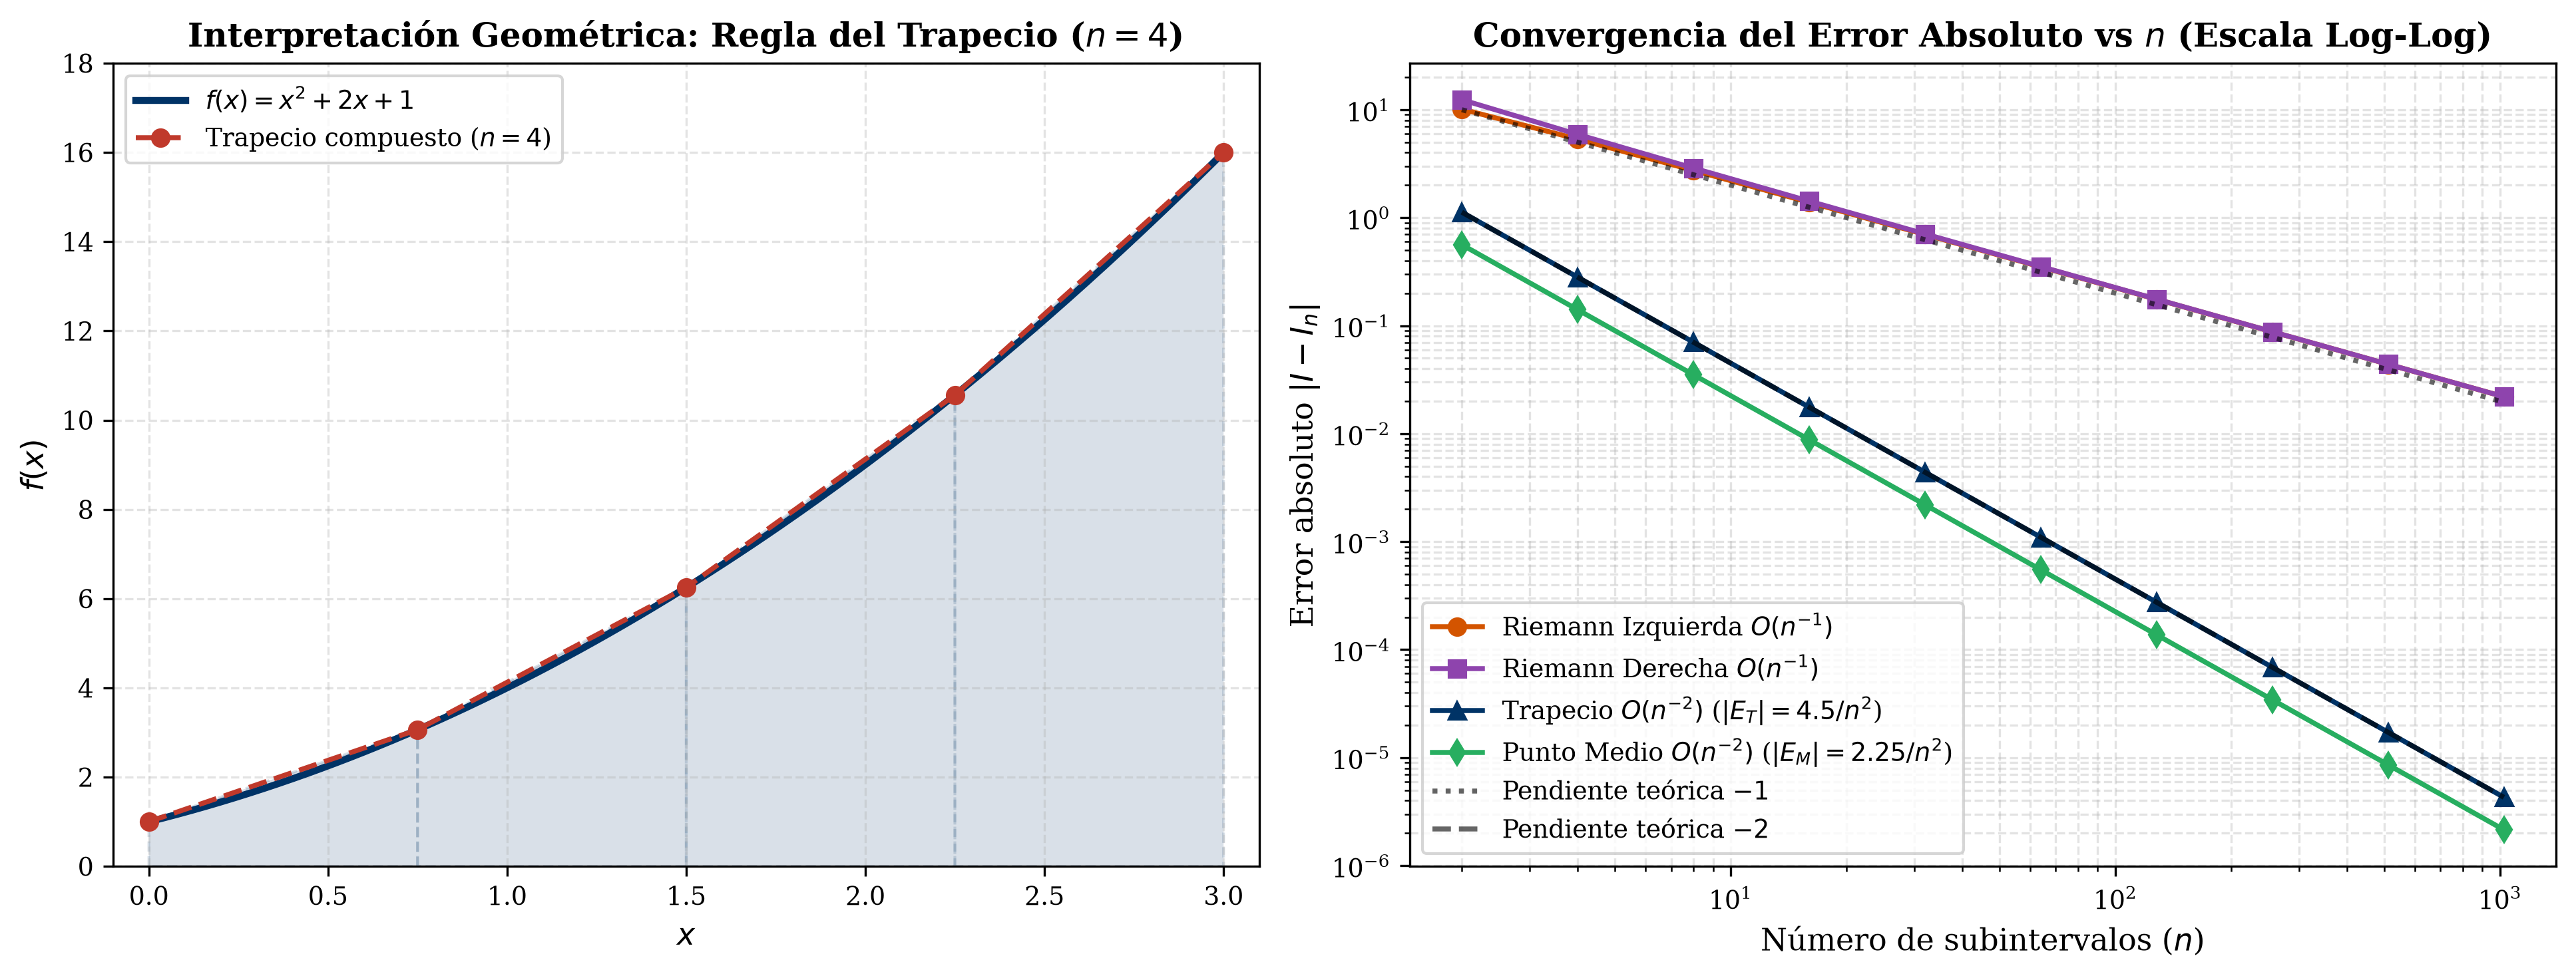
\includegraphics[width=0.98\textwidth]{fig_ejercicio1_convergencia.png}
    \caption{Ejercicio 1: (Izquierda) Interpretación geométrica de los trapecios sobre $f(x) = x^2+2x+1$ para $n=4$. (Derecha) Gráfica log-log de convergencia de los cuatro métodos mostrando órdenes $O(n^{-1})$ y $O(n^{-2})$.}
    \label{fig:ejercicio1}
\end{figure}

% ==============================================================================
% EJERCICIO 2
% ==============================================================================
\section{Ejercicio 2: Función trigonométrica}

Considere la integral:
\begin{equation}
    I = \int_0^\pi \sin(x)\, dx.
\end{equation}

\subsection{1. Valor exacto analítico}
Integrando directamente:
\begin{equation}
    I = [-\cos(x)]_0^\pi = -\cos(\pi) - (-\cos(0)) = -(-1) - (-1) = 1 + 1 = \mathbf{2}.
\end{equation}

\subsection{2. Aproximación con los métodos estudiados}
En la Tabla~\ref{tab:ejercicio2_errores} se presentan las aproximaciones numéricas para $n = 2, 4, 8, 16, 32, 64, 128, 256$.

\begin{table}[h!]
\centering
\caption{Aproximaciones y errores absolutos para $I = \int_0^\pi \sin(x)\, dx = 2$.}
\label{tab:ejercicio2_errores}
\begin{tabular}{rcccccc}
\toprule
$n$ & Trapecio $T(n)$ & Error $T(n)$ & Punto Medio $M(n)$ & Error $M(n)$ & Riemann Izq. $R_L(n)$ & Error $R_L(n)$ \\
\midrule
2   & $1.57079633$ & $4.2920\times 10^{-1}$ & $2.22144147$ & $2.2144\times 10^{-1}$ & $1.57079633$ & $4.2920\times 10^{-1}$ \\
4   & $1.89611890$ & $1.0388\times 10^{-1}$ & $2.05234431$ & $5.2344\times 10^{-2}$ & $1.89611890$ & $1.0388\times 10^{-1}$ \\
8   & $1.97423160$ & $2.5768\times 10^{-2}$ & $2.01290909$ & $1.2909\times 10^{-2}$ & $1.97423160$ & $2.5768\times 10^{-2}$ \\
16  & $1.99357034$ & $6.4297\times 10^{-3}$ & $2.00321638$ & $3.2164\times 10^{-3}$ & $1.99357034$ & $6.4297\times 10^{-3}$ \\
32  & $1.99839336$ & $1.6066\times 10^{-3}$ & $2.00080342$ & $8.0342\times 10^{-4}$ & $1.99839336$ & $1.6066\times 10^{-3}$ \\
64  & $1.99959839$ & $4.0161\times 10^{-4}$ & $2.00020081$ & $2.0081\times 10^{-4}$ & $1.99959839$ & $4.0161\times 10^{-4}$ \\
128 & $1.99989960$ & $1.0040\times 10^{-4}$ & $2.00005020$ & $5.0200\times 10^{-5}$ & $1.99989960$ & $1.0040\times 10^{-4}$ \\
256 & $1.99997490$ & $2.5100\times 10^{-5}$ & $2.00001255$ & $1.2550\times 10^{-5}$ & $1.99997490$ & $2.5100\times 10^{-5}$ \\
\bottomrule
\end{tabular}
\end{table}

\subsection{3. Análisis del efecto de incrementar $n$ y propiedades de simetría}
Al analizar la Tabla~\ref{tab:ejercicio2_errores} se revelan comportamientos numéricos fundamentales:

\begin{enumerate}
    \item \textbf{Identidad entre Riemann Izquierda, Riemann Derecha y Trapecio:}
    Observe que los valores numéricos de $R_L(n)$, $R_R(n)$ y $T(n)$ son idénticos. Esto no es una coincidencia numérica, sino una propiedad algebraica directa de los extremos del intervalo:
    \begin{equation}
        f(0) = \sin(0) = 0, \qquad f(\pi) = \sin(\pi) = 0.
    \end{equation}
    Por definición:
    \begin{align}
        R_L(n) &= h \left[ f(0) + \sum_{i=1}^{n-1} f(x_i) \right] = h \sum_{i=1}^{n-1} \sin(x_i), \\
        R_R(n) &= h \left[ \sum_{i=1}^{n-1} f(x_i) + f(\pi) \right] = h \sum_{i=1}^{n-1} \sin(x_i), \\
        T(n)   &= \frac{h}{2} [f(0) + f(\pi)] + h \sum_{i=1}^{n-1} f(x_i) = h \sum_{i=1}^{n-1} \sin(x_i).
    \end{align}
    Por lo tanto, $R_L(n) \equiv R_R(n) \equiv T(n)$ para toda partición uniforme.

    \item \textbf{Aceleración de convergencia por la fórmula de Euler-Maclaurin:}
    Normalmente las sumas de Riemann convergen a orden 1 ($O(n^{-1})$). Sin embargo, al anularse los extremos de frontera, la fórmula de Euler-Maclaurin establece:
    \begin{equation}
        T(h) - I = \frac{h^2}{12} \left[ f'(\pi) - f'(0) \right] - \frac{h^4}{720} \left[ f'''(\pi) - f'''(0) \right] + \dots
    \end{equation}
    Como $f'(x) = \cos(x)$, se tiene $f'(0) = 1$ y $f'(\pi) = -1$:
    \begin{equation}
        T(h) - I = \frac{h^2}{12} (-1 - 1) + O(h^4) = -\frac{h^2}{6} + O(h^4) = -\frac{\pi^2}{6 n^2} + O(n^{-4}).
    \end{equation}
    ¡El error de la regla del trapecio (y de las sumas de Riemann para esta función) decae con orden cuadrático $O(n^{-2})$! La constante asintótica es $\frac{\pi^2}{6 n^2} \approx \frac{1.6449}{n^2}$.
    
    \item \textbf{Orden experimental de convergencia:}
    Calculando $p \approx \log_2(E_n / E_{2n})$ a partir de la Tabla~\ref{tab:ejercicio2_errores}:
    \begin{equation}
        p_{2\to 4} = 2.0467, \quad p_{4\to 8} = 2.0113, \quad p_{8\to 16} = 2.0028, \quad p_{16\to 32} = 2.0007, \quad p_{128\to 256} = 2.0000.
    \end{equation}
    El orden converge exactamente a $2$, lo que corrobora la predicción teórica.
\end{enumerate}

\subsection{4. Gráfica del error absoluto del trapecio en función de $n$}
En la Figura~\ref{fig:ejercicio2} se grafican los errores en escala lineal y escala logarítmica, mostrando la concordancia perfecta con la asíntota de Euler-Maclaurin.

\begin{figure}[h!]
    \centering
    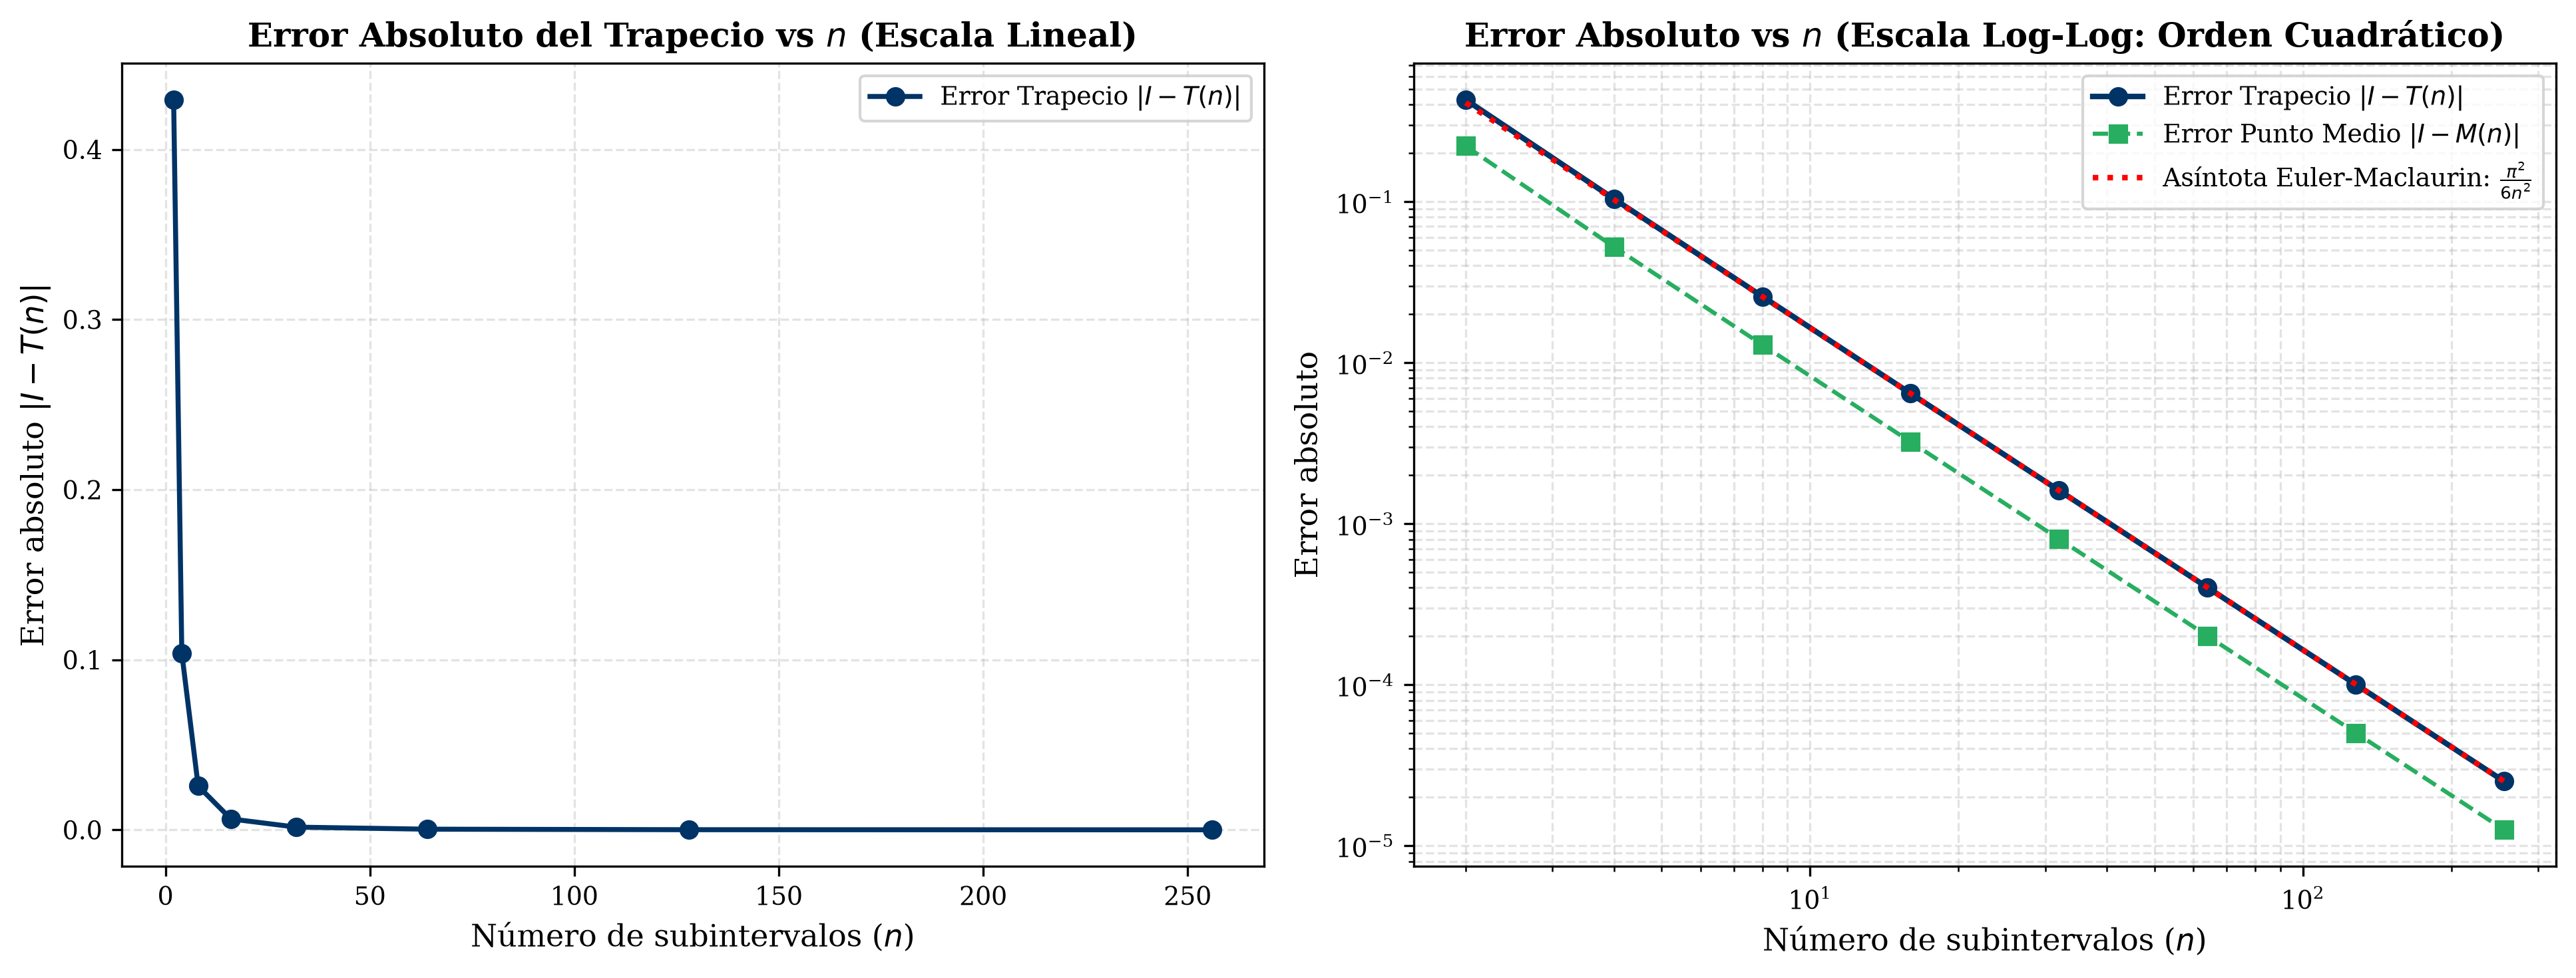
\includegraphics[width=0.98\textwidth]{fig_ejercicio2_error_trapecio.png}
    \caption{Ejercicio 2: (Izquierda) Error absoluto del trapecio vs $n$ en escala lineal. (Derecha) Gráfica log-log comparando el error del trapecio y del punto medio con la asíntota teórica $\frac{\pi^2}{6 n^2}$.}
    \label{fig:ejercicio2}
\end{figure}

% ==============================================================================
% EJERCICIO 3
% ==============================================================================
\section{Ejercicio 3: Exponencial}

Considere la integral definida:
\begin{equation}
    I = \int_0^2 e^x\, dx.
\end{equation}

\subsection{1. Valor exacto analítico}
Integrando la función exponencial:
\begin{equation}
    I = [e^x]_0^2 = e^2 - e^0 = e^2 - 1 \approx \mathbf{6.3890560989}.
\end{equation}

\subsection{2. Comparación entre la regla del trapecio y rectángulos}
La función $f(x) = e^x$ es estrictamente creciente ($f'(x) = e^x > 0$) y estrictamente convexa ($f''(x) = e^x > 0$) en todo $[0, 2]$.

\begin{itemize}[leftmargin=*]
    \item \textbf{Rectángulos por izquierda ($R_L$):} Subestima la integral en cada intervalo porque $f(x) \ge f(x_i)$ para $x \in [x_i, x_{i+1}]$. El error asintótico es:
    \begin{equation}
        E_{R_L} \approx \frac{h}{2} [f(b) - f(a)] = \frac{e^2 - 1}{n} = O(n^{-1}).
    \end{equation}
    \item \textbf{Rectángulos por derecha ($R_R$):} Sobreestima sistemáticamente el área:
    \begin{equation}
        E_{R_R} \approx -\frac{h}{2} [f(b) - f(a)] = -\frac{e^2 - 1}{n} = O(n^{-1}).
    \end{equation}
    \item \textbf{Regla del trapecio ($T$):} Las secantes quedan por encima de la curva exponencial convexa, produciendo una sobreestimación con orden cuadrático $O(n^{-2})$:
    \begin{equation}
        E_T = -\frac{(b-a)^3}{12 n^2} f''(\xi) = -\frac{8}{12 n^2} e^\xi = -\frac{2}{3 n^2} e^\xi, \qquad \xi \in (0, 2).
    \end{equation}
    \item \textbf{Regla del punto medio ($M$):} Las tangentes en el centro quedan por debajo de la curva convexa, subestimando la integral con la mitad del error del trapecio:
    \begin{equation}
        E_M = \frac{(b-a)^3}{24 n^2} f''(\eta) = \frac{1}{3 n^2} e^\eta, \qquad \eta \in (0, 2).
    \end{equation}
\end{itemize}

\subsection{3. Determinación del número de subintervalos para tolerancia $10^{-6}$}
Deseamos encontrar $n$ tal que el error absoluto sea estrictamente menor que $\varepsilon = 10^{-6}$.

\paragraph{A) Cotas teóricas a priori (conservadoras):}
Como $f''(x) = e^x$ alcanza su máximo en el extremo derecho $x=2$, $M_2 = \max_{x\in[0,2]} |f''(x)| = e^2 \approx 7.389056$:
\begin{itemize}
    \item \textbf{Trapecio:}
    \begin{equation}
        |E_T| \le \frac{2 e^2}{3 n^2} \le 10^{-6} \implies n \ge \sqrt{\frac{2 e^2 \times 10^6}{3}} \approx \sqrt{4{,}926{,}037} \approx 2219.46 \implies \mathbf{n \ge 2220}.
    \end{equation}
    \item \textbf{Punto Medio:}
    \begin{equation}
        |E_M| \le \frac{e^2}{3 n^2} \le 10^{-6} \implies n \ge \sqrt{\frac{e^2 \times 10^6}{3}} \approx \sqrt{2{,}463{,}018} \approx 1569.40 \implies \mathbf{n \ge 1570}.
    \end{equation}
    \item \textbf{Rectángulos:} Con $M_1 = \max |f'(x)| = e^2$:
    \begin{equation}
        |E_R| \le \frac{(b-a)^2}{2n} M_1 = \frac{2 e^2}{n} \le 10^{-6} \implies n \ge 2 e^2 \times 10^6 \approx \mathbf{14{,}778{,}112}.
    \end{equation}
\end{itemize}

\paragraph{B) Mínimo número de subintervalos real computacional:}
La cota teórica es conservadora porque asume que $f''(\xi) = e^2$ en todos los intervalos. Por la fórmula de Euler-Maclaurin, el error medio asintótico está gobernado por:
\begin{equation}
    E_T \approx \frac{h^2}{12} [f'(2) - f'(0)] = \frac{4}{12 n^2} (e^2 - 1) = \frac{e^2 - 1}{3 n^2}.
\end{equation}
Exigiendo $\frac{e^2 - 1}{3 n^2} < 10^{-6}$ se obtiene la estimación:
\begin{equation}
    n > \sqrt{\frac{(e^2 - 1) \times 10^6}{3}} \approx \sqrt{2{,}129{,}685} \approx 1459.34 \implies n = 1460.
\end{equation}
La búsqueda computacional directa en Python confirma los valores mínimos exactos:
\begin{itemize}
    \item \textbf{Trapecio:} $\mathbf{n = 1460}$ (con error exacto de $9.9910 \times 10^{-7} < 10^{-6}$).
    \item \textbf{Punto Medio:} $\mathbf{n = 1032}$ (con error exacto de $9.9983 \times 10^{-7} < 10^{-6}$).
    \item \textbf{Rectángulos:} $\mathbf{n = 6{,}389{,}057}$ ($\sim 6.39$ millones de subintervalos).
\end{itemize}

El método del trapecio requiere \textbf{4376 veces menos subintervalos} que los rectángulos para alcanzar una precisión de 6 cifras decimales, demostrando la superioridad abrumadora de los métodos de orden 2. En la Figura~\ref{fig:ejercicio3} se aprecia la intersección con el umbral de tolerancia.

\begin{figure}[h!]
    \centering
    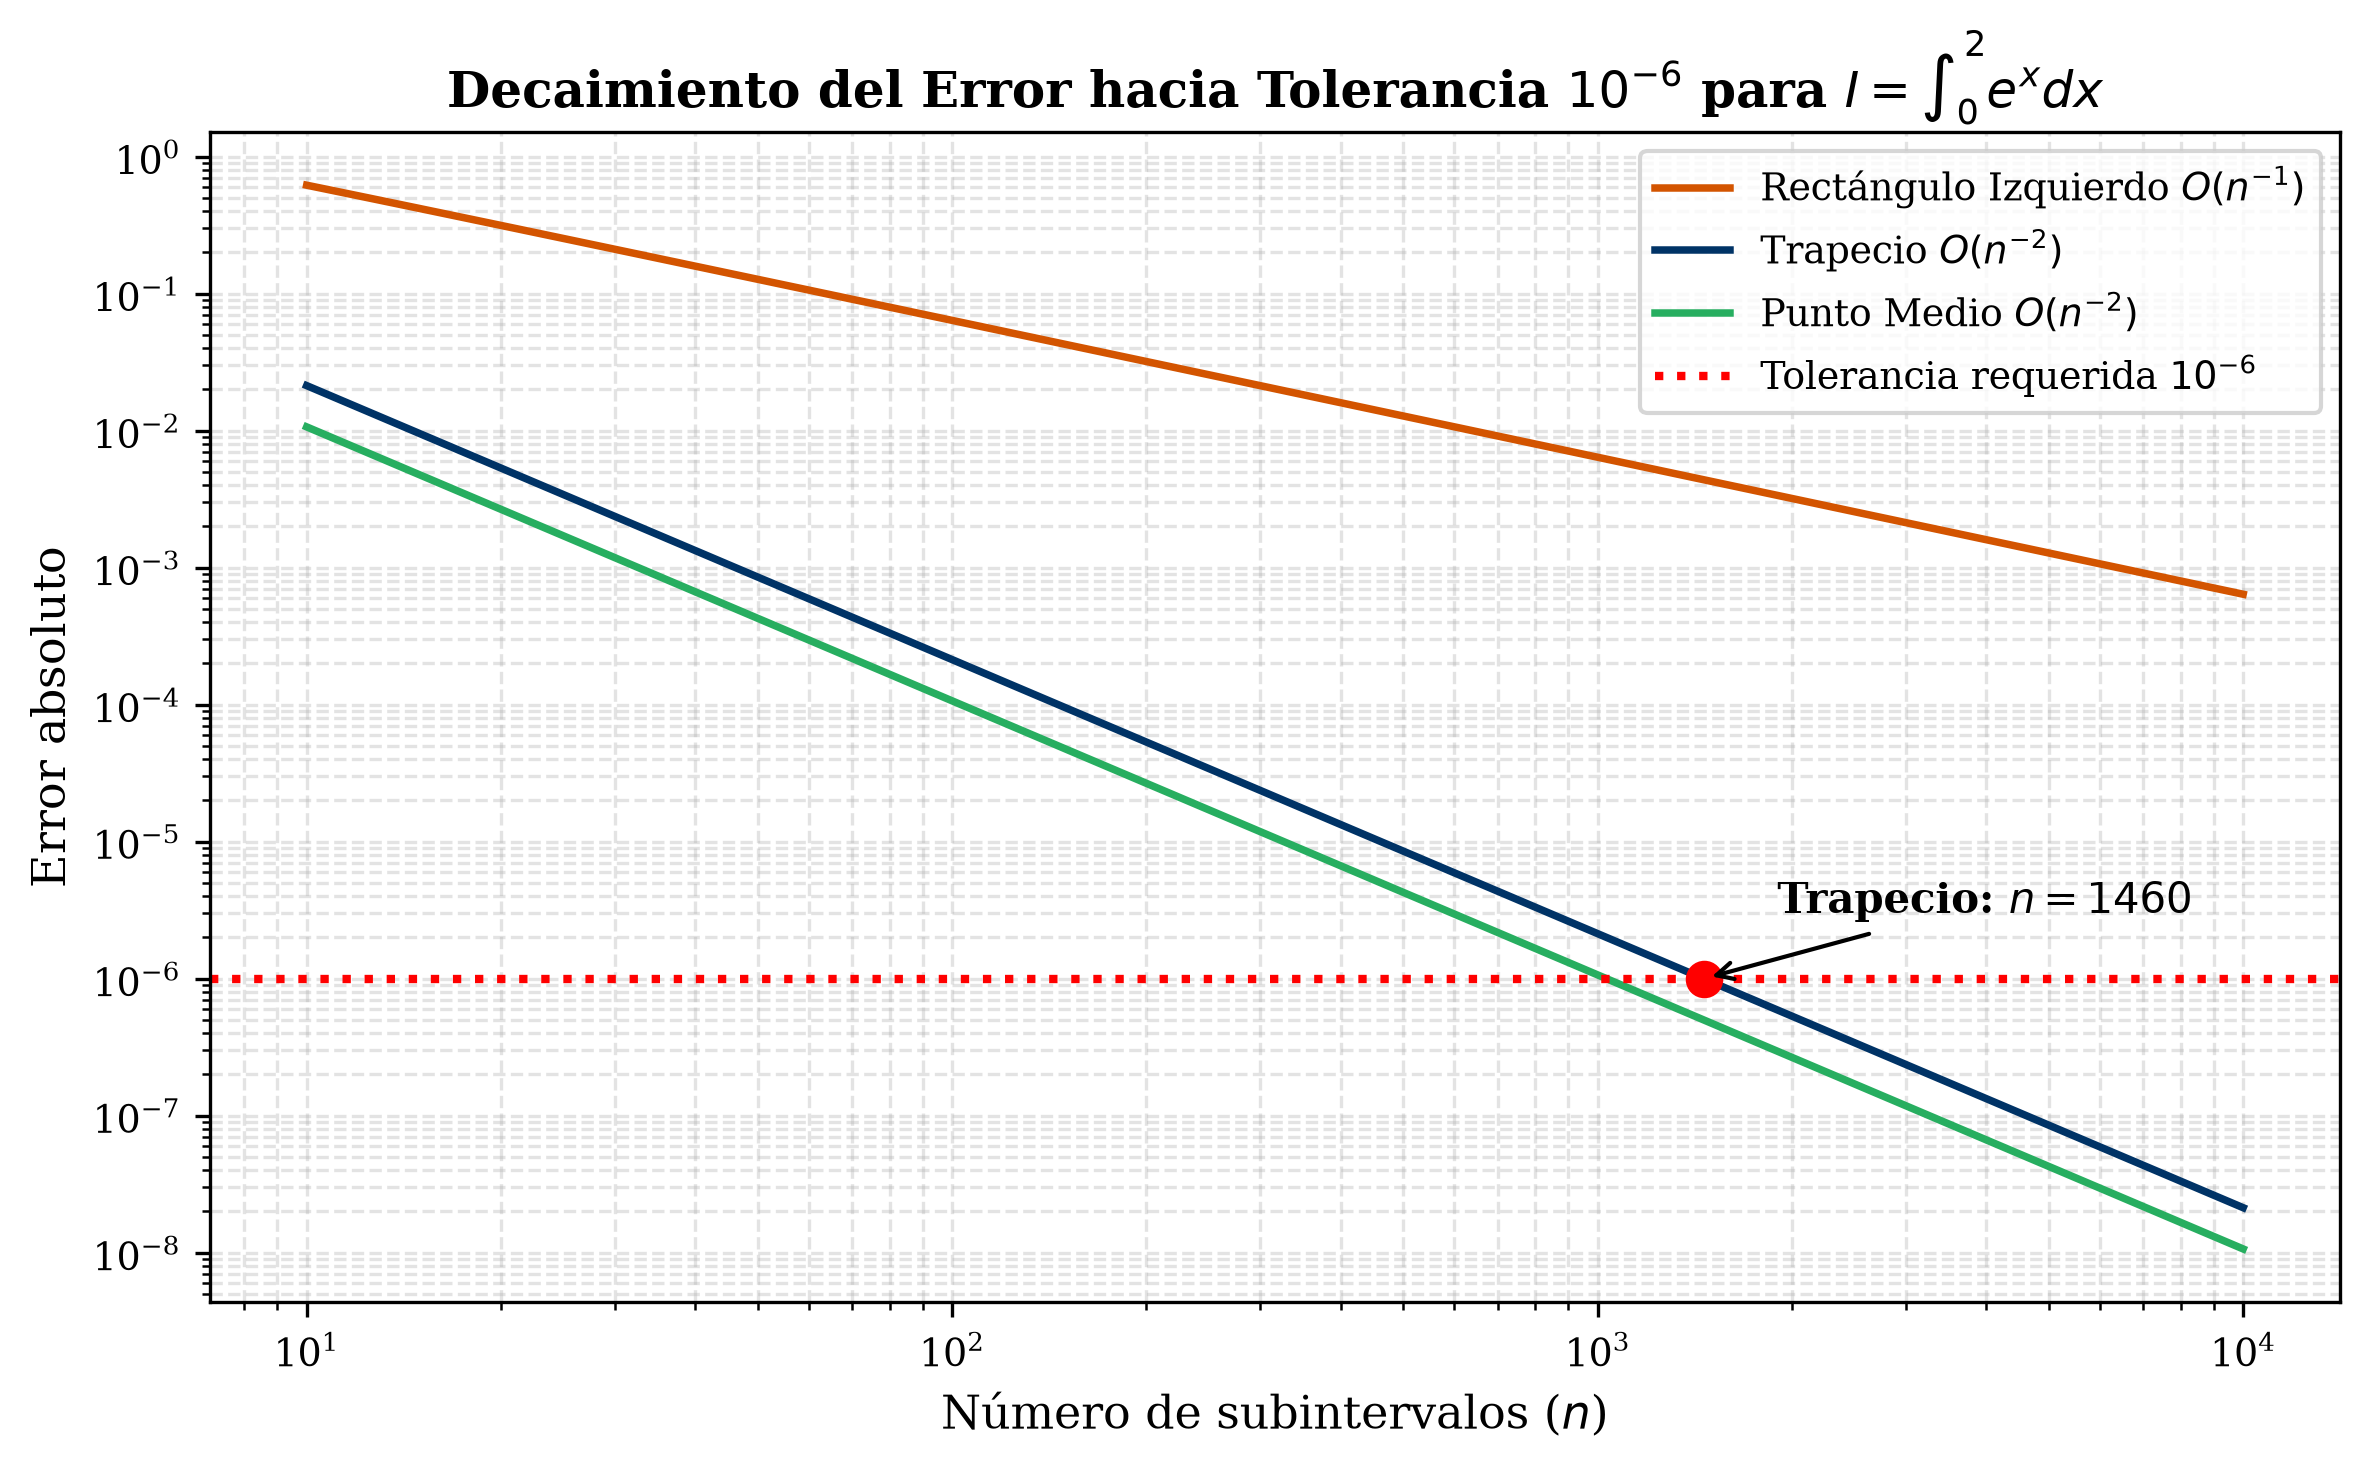
\includegraphics[width=0.72\textwidth]{fig_ejercicio3_exponencial.png}
    \caption{Ejercicio 3: Trayectoria de error hacia la tolerancia $10^{-6}$ para $I = \int_0^2 e^x\, dx$.}
    \label{fig:ejercicio3}
\end{figure}

% ==============================================================================
% EJERCICIO 4
% ==============================================================================
\section{Ejercicio 4: Datos experimentales}

Un experimento produce los siguientes datos discretos aproximados de una función desconocida:
\begin{table}[h!]
\centering
\begin{tabular}{ccccc}
\toprule
$x$ & $0$ & $1$ & $2$ & $3$ \\
$f(x)$ & $1.0$ & $1.8$ & $2.4$ & $4.1$ \\
\bottomrule
\end{tabular}
\end{table}

Los nodos están equiespaciados con paso constante $h = 1$ y $n = 3$ subintervalos: $[0, 1]$, $[1, 2]$ y $[2, 3]$.

\subsection{1. Aproximación de la integral}

\begin{itemize}[leftmargin=*]
    \item \textbf{Regla del Trapecio compuesta:}
    \begin{align}
        T &= \frac{h}{2} \left[ f(x_0) + 2 f(x_1) + 2 f(x_2) + f(x_3) \right] \nonumber \\
          &= \frac{1}{2} \left[ 1.0 + 2(1.8) + 2(2.4) + 4.1 \right] \nonumber \\
          &= \frac{1}{2} \left[ 1.0 + 3.6 + 4.8 + 4.1 \right] = \frac{13.5}{2} = \mathbf{6.75}.
    \end{align}

    \item \textbf{Rectángulos por la izquierda ($R_L$):}
    \begin{equation}
        R_L = h \left[ f(x_0) + f(x_1) + f(x_2) \right] = 1.0 \times [1.0 + 1.8 + 2.4] = \mathbf{5.20}.
    \end{equation}

    \item \textbf{Rectángulos por la derecha ($R_R$):}
    \begin{equation}
        R_R = h \left[ f(x_1) + f(x_2) + f(x_3) \right] = 1.0 \times [1.8 + 2.4 + 4.1] = \mathbf{8.30}.
    \end{equation}
\end{itemize}

Observe que el promedio de las aproximaciones rectangulares coincide exactamente con el trapecio: $\frac{R_L + R_R}{2} = \frac{5.20 + 8.30}{2} = 6.75$. Además, como $n=3$ no es par, no se puede aplicar Simpson 1/3 clásico, pero aplicando la regla de Simpson 3/8 para 3 subintervalos:
\begin{equation}
    S_{3/8} = \frac{3h}{8} [f_0 + 3f_1 + 3f_2 + f_3] = \frac{3}{8} [1.0 + 5.4 + 7.2 + 4.1] = \frac{3 \times 17.7}{8} = \mathbf{6.6375}.
\end{equation}

\subsection{2. Discusión de las limitaciones de integrar datos experimentales}
Integrar datos experimentales impone serias limitaciones físicas y matemáticas respecto a la integración de funciones analíticas:

\begin{enumerate}[leftmargin=*]
    \item \textbf{Imposibilidad de refinamiento de malla ($h \to 0$):}
    A diferencia de una función matemática donde el analista puede reducir $h$ a voluntad para satisfacer una tolerancia prefijada, en datos experimentales el espaciado $h$ viene impuesto por la instrumentación del ensayo. No es posible generar nuevos datos sin realizar nuevos experimentos.

    \item \textbf{Propagación de incertidumbre y ruido de medición:}
    Las mediciones reales contienen ruido: $\tilde{y}_i = y_i + \varepsilon_i$, donde $\varepsilon_i \sim \mathcal{N}(0, \sigma^2)$. Para el trapecio, la varianza de la integral resultante es:
    \begin{equation}
        \mathrm{Var}(T) = \frac{h^2}{4} \left[ \sigma^2 + 4\sigma^2 + 4\sigma^2 + \sigma^2 \right] = 2.5\, h^2 \sigma^2.
    \end{equation}
    Aunque la integración actúa como filtro paso-bajo que suaviza el ruido aleatorio (a diferencia de la diferenciación numérica que lo amplifica catastróficamente), el sesgo instrumental sistemático no se elimina.

    \item \textbf{Inaccesibilidad de nodos intermedios y métodos de alto orden:}
    Métodos como la regla del punto medio requieren conocer $f(0.5)$, $f(1.5)$, $f(2.5)$, los cuales no fueron muestreados. Para emplearlos se requeriría recurrir a una etapa previa de interpolación (por ejemplo, splines cúbicos), introduciendo un error de modelo adicional.

    \item \textbf{Desconocimiento de las derivadas y cotas de error de truncamiento:}
    Al no existir una función analítica $f(x)$, resulta imposible evaluar $f''(\xi)$ para calcular cotas teóricas rigurosas sobre el error de truncamiento. Solo se pueden hacer estimaciones cualitativas basadas en diferencias finitas.
\end{enumerate}

En la Figura~\ref{fig:ejercicio4} se representan las áreas integradas bajo cada esquema.

\begin{figure}[h!]
    \centering
    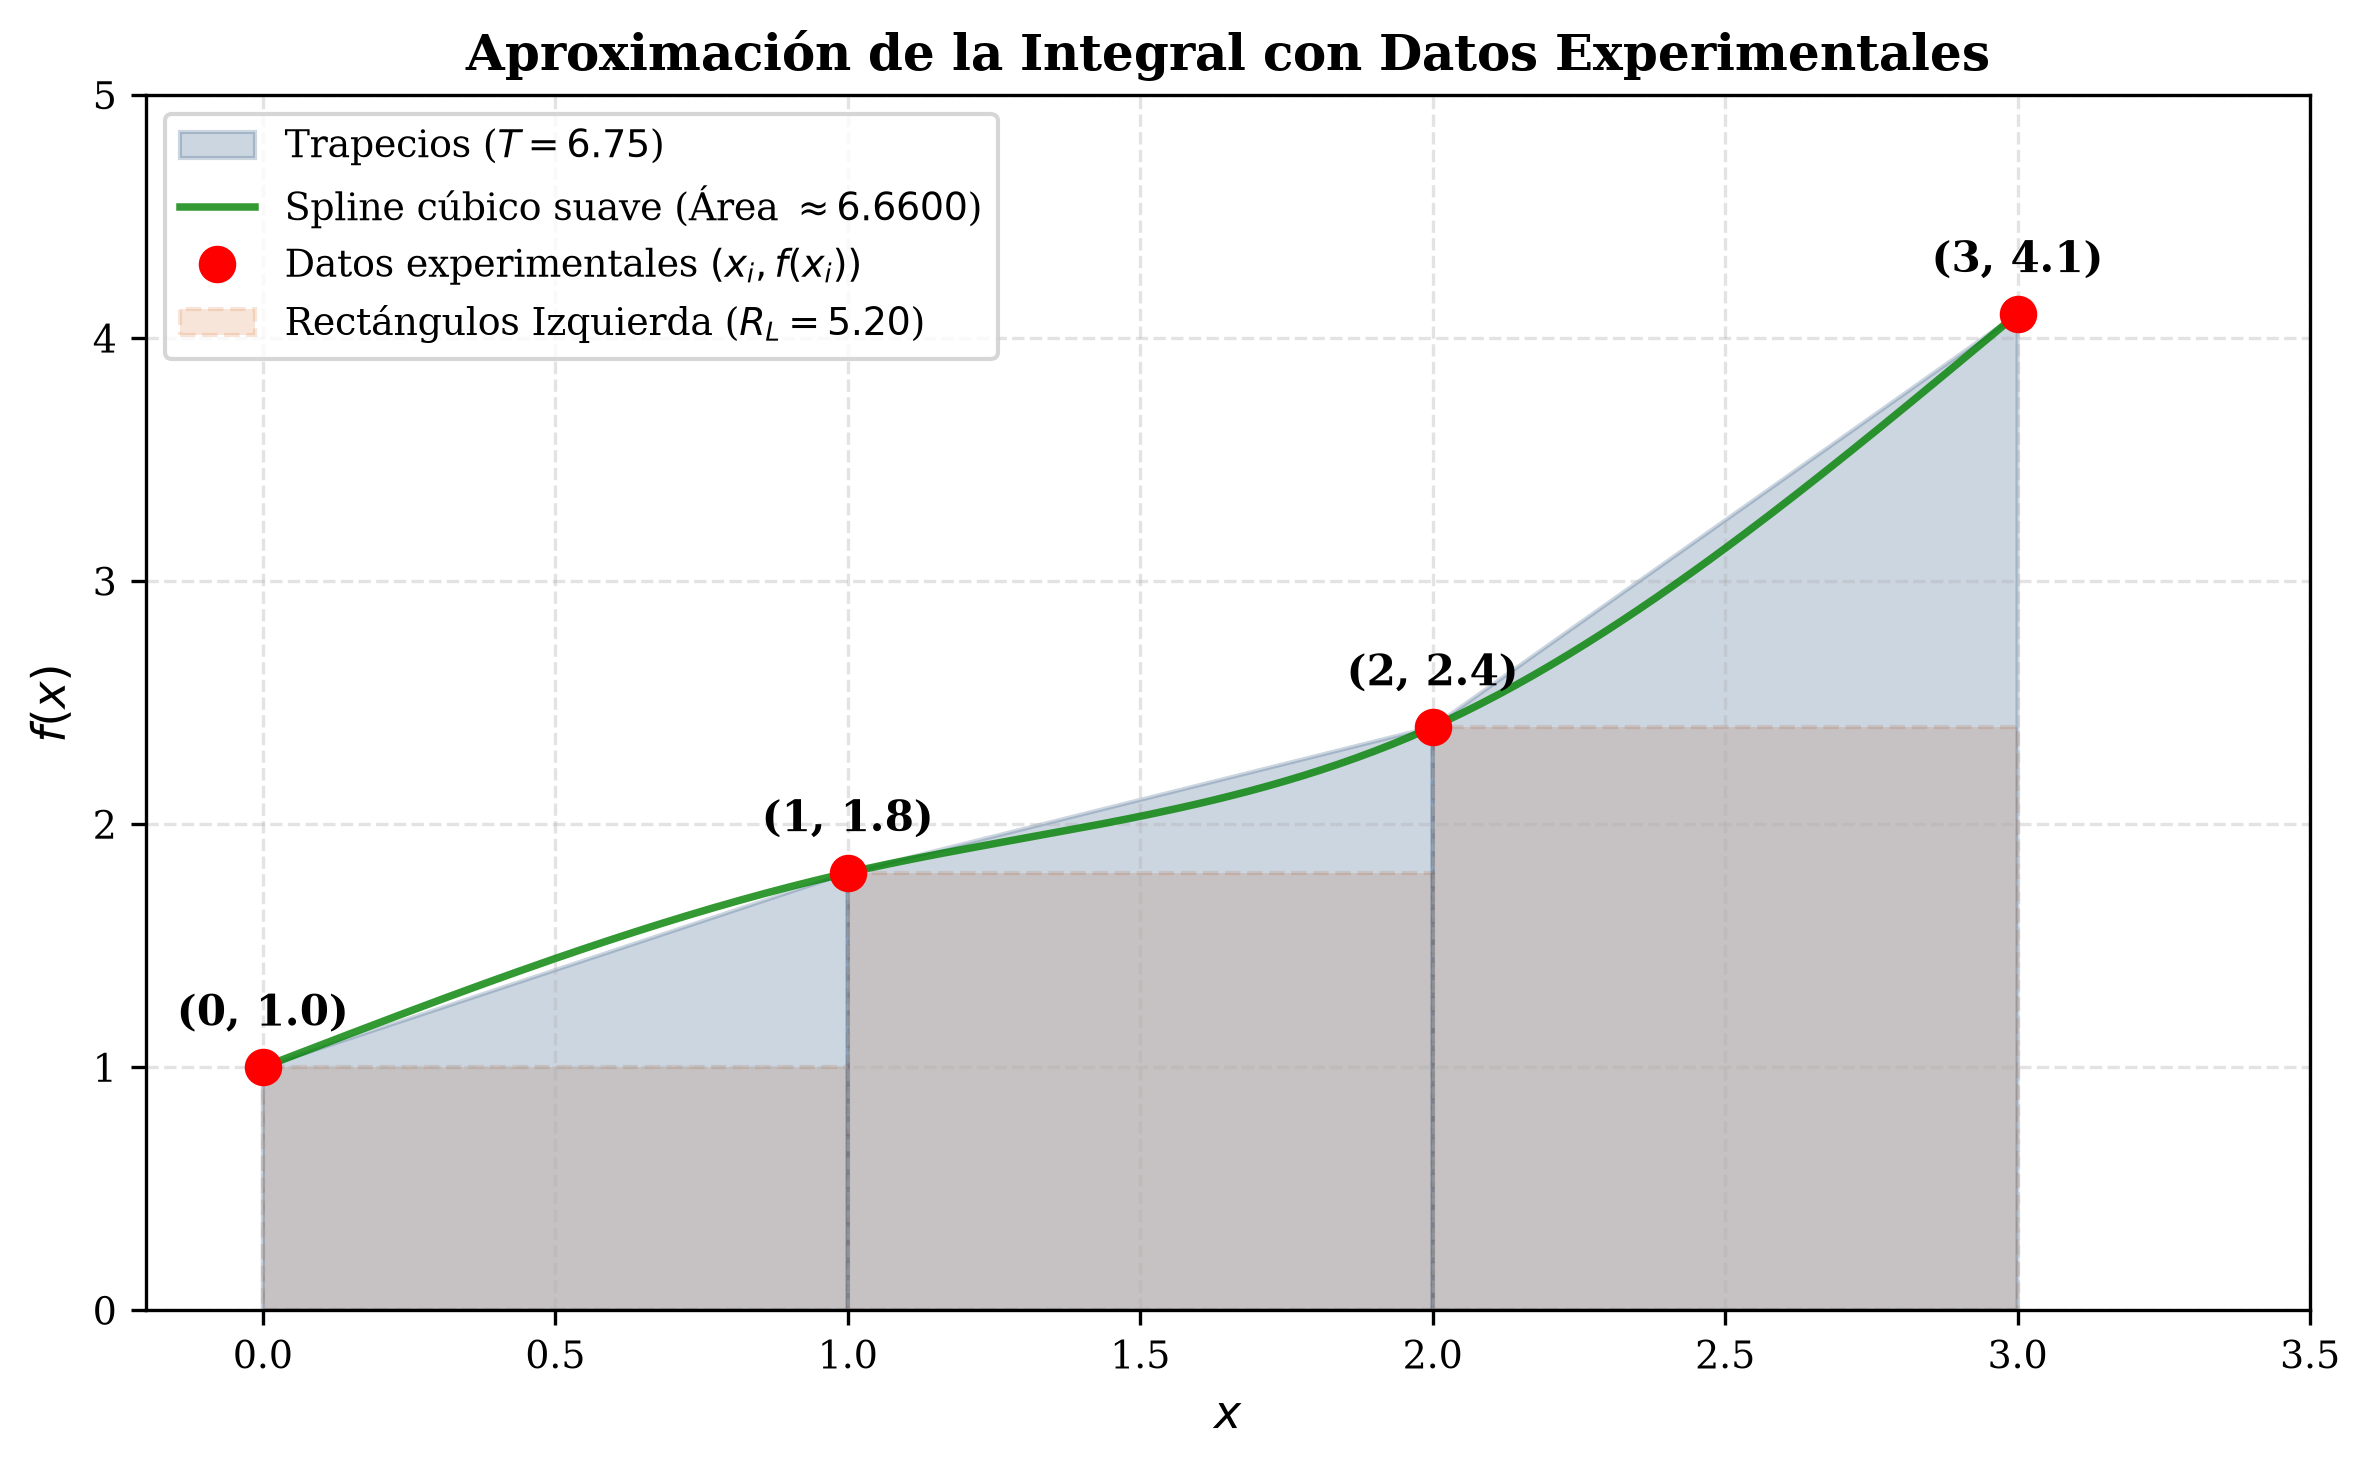
\includegraphics[width=0.75\textwidth]{fig_ejercicio4_datos_experimentales.png}
    \caption{Ejercicio 4: Integración de datos experimentales discretos mediante trapecios, rectángulos y spline cúbico natural interpolante.}
    \label{fig:ejercicio4}
\end{figure}

% ==============================================================================
% EJERCICIO 5
% ==============================================================================
\section{Ejercicio 5: Oscilaciones de alta frecuencia}

Considere la integral definida:
\begin{equation}
    I = \int_0^1 e^{-x} \sin(40x^2 + 5x)\, dx.
\end{equation}

\subsection{1. Gráfica de la función e identificación de regiones de mayor oscilación}
Sea el argumento del seno la función de fase $\theta(x) = 40x^2 + 5x$. La frecuencia angular instantánea $\omega(x)$ se define como la derivada temporal/espacial de la fase:
\begin{equation}
    \omega(x) = \frac{d\theta}{dx} = 80x + 5 \quad [\text{rad/unid}].
\end{equation}
Evaluando en los extremos del intervalo $[0, 1]$:
\begin{align}
    \omega(0) &= 80(0) + 5 = 5 \text{ rad/unid} \implies \text{Longitud de onda local } \lambda(0) = \frac{2\pi}{5} \approx 1.257, \\
    \omega(1) &= 80(1) + 5 = 85 \text{ rad/unid} \implies \text{Longitud de onda local } \lambda(1) = \frac{2\pi}{85} \approx 0.0739.
\end{align}
La frecuencia instantánea \textbf{se multiplica por un factor de 17} a lo largo del intervalo. Por consiguiente, la región de mayor oscilación se concentra marcadamente en el extremo derecho $x \to 1$, donde la longitud de onda se reduce a solo $0.0739$, mientras que cerca de $x=0$ la función varía con relativa suavidad modulada por la envolvente exponencial $e^{-x}$ (ver Figura~\ref{fig:ejercicio5}(a)).

\subsection{2--4. Aproximación, errores absolutos y convergencia}
Para calcular el error absoluto real se calculó previamente una referencia numérica de alta precisión mediante cuadratura adaptativa Gauss-Kronrod (\texttt{scipy.integrate.quad} con tolerancias estrictas $10^{-14}$):
\begin{equation}
    I_{\text{ref}} = \mathbf{0.079770893293}.
\end{equation}

En la Tabla~\ref{tab:ejercicio5} se comparan las aproximaciones y errores de la regla del trapecio y de la regla de Simpson 1/3 para los subintervalos indicados: $n = 20, 40, 80, 160, 320$.

\begin{table}[h!]
\centering
\caption{Comparación entre Trapecio y Simpson 1/3 para la integral con oscilaciones de alta frecuencia.}
\label{tab:ejercicio5}
\begin{tabular}{rcccc}
\toprule
$n$ & Trapecio $T(n)$ & Error Absoluto Trapecio & Simpson 1/3 $S(n)$ & Error Absoluto Simpson 1/3 \\
\midrule
20  & $0.08411394$ & $4.3430\times 10^{-3}$ & $0.13156848$ & $5.1798\times 10^{-2}$ \\
40  & $0.08042234$ & $6.5145\times 10^{-4}$ & $0.07919181$ & $5.7908\times 10^{-4}$ \\
80  & $0.07991972$ & $1.4883\times 10^{-4}$ & $0.07975218$ & $1.8711\times 10^{-5}$ \\
160 & $0.07980732$ & $3.6429\times 10^{-5}$ & $0.07976986$ & $1.0377\times 10^{-6}$ \\
320 & $0.07977995$ & $9.0600\times 10^{-6}$ & $0.07977083$ & $6.3060\times 10^{-8}$ \\
\bottomrule
\end{tabular}
\end{table}

\subsection{5. Estimación del orden experimental de convergencia}
El orden experimental de convergencia entre dos particiones sucesivas con paso $h_1$ y $h_2 = h_1 / 2$ se calcula mediante:
\begin{equation}
    p = \frac{\ln(E_{n_1} / E_{n_2})}{\ln(n_2 / n_1)} = \log_2\left( \frac{E(n)}{E(2n)} \right).
\end{equation}
Aplicando esta fórmula a los datos de la Tabla~\ref{tab:ejercicio5}:
\begin{itemize}
    \item \textbf{Intervalo $n \in [20, 40]$:} $p_{\text{Trap}} = 2.74$, \quad $p_{\text{Simp}} = 6.48$. (Régimen pre-asintótico: con $n=20$, $h = 0.05$ es cercano a la longitud de onda crítica $\lambda(1) \approx 0.074$, provocando submuestreo severo en Simpson).
    \item \textbf{Intervalo $n \in [40, 80]$:} $p_{\text{Trap}} = 2.13$, \quad $p_{\text{Simp}} = 4.95$.
    \item \textbf{Intervalo $n \in [80, 160]$:} $p_{\text{Trap}} = 2.03$, \quad $p_{\text{Simp}} = 4.17$.
    \item \textbf{Intervalo $n \in [160, 320]$:} $p_{\text{Trap}} = \mathbf{2.01} \approx 2$, \quad $p_{\text{Simp}} = \mathbf{4.04} \approx 4$.
\end{itemize}
Una vez que el tamaño del paso $h$ resuelve adecuadamente cada ciclo oscilatorio ($n \ge 80$), ambos algoritmos ingresan plenamente en el régimen asintótico, confirmando experimentalmente los órdenes teóricos $p=2$ para Trapecio y $p=4$ para Simpson 1/3.

\subsection{6. Menor número de subintervalos para tolerancia $10^{-6}$}
Buscando computacionalmente el primer valor de $n$ que cumple $|I_{\text{ref}} - I_n| < 10^{-6}$:
\begin{itemize}
    \item \textbf{Regla del Trapecio:} Requiere $\mathbf{n = 963}$ subintervalos ($h \approx 1.038 \times 10^{-3}$, Error $= 9.9886 \times 10^{-7}$).
    \item \textbf{Regla de Simpson 1/3:} Requiere únicamente $\mathbf{n = 162}$ subintervalos ($h \approx 6.173 \times 10^{-3}$, Error $= 9.8647 \times 10^{-7}$).
\end{itemize}
Gracias a su convergencia cuártica ($O(h^4)$), Simpson 1/3 alcanza la tolerancia de $10^{-6}$ con casi \textbf{6 veces menos subintervalos} y evaluaciones de función que el método del trapecio.

\begin{figure}[h!]
    \centering
    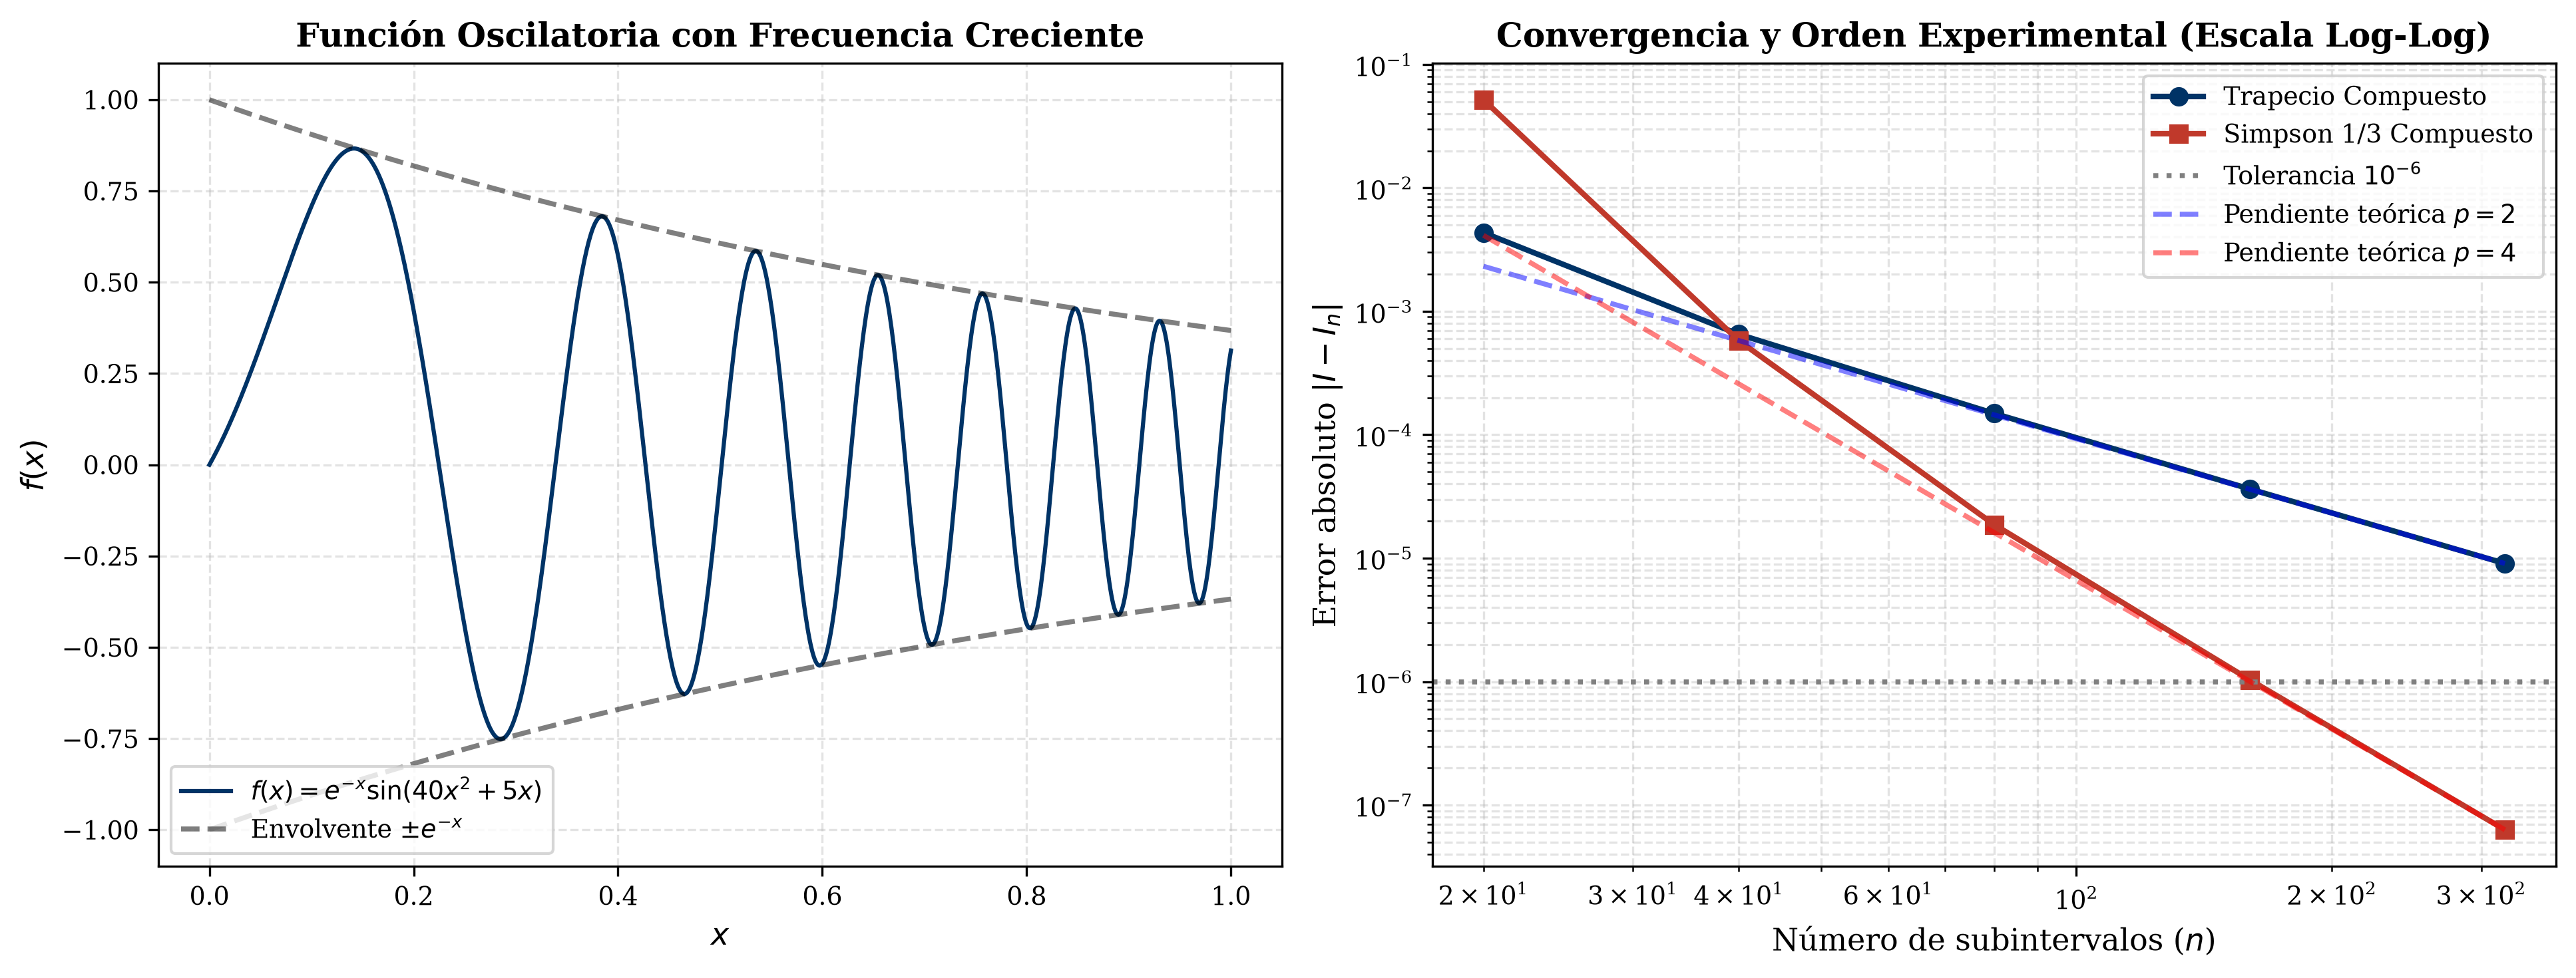
\includegraphics[width=0.98\textwidth]{fig_ejercicio5_oscilaciones.png}
    \caption{Ejercicio 5: (Izquierda) Señal oscilatoria modulada y envolventes $\pm e^{-x}$. (Derecha) Gráfica log-log de convergencia mostrando la transición al régimen asintótico y pendientes teóricas $p=2$ y $p=4$.}
    \label{fig:ejercicio5}
\end{figure}

% ==============================================================================
% EJERCICIO 6
% ==============================================================================
\section{Ejercicio 6: Integral altamente oscilatoria}

Considere la integral definida:
\begin{equation}
    I = \int_0^1 \sin\left( \frac{1}{x + 0.01} \right)\, dx.
\end{equation}

\subsection{1. Frecuencia de oscilación a lo largo del intervalo}
La fase de la función es $\theta(x) = \frac{1}{x + 0.01}$. Su frecuencia instantánea es:
\begin{equation}
    \omega(x) = \left| \frac{d\theta}{dx} \right| = \frac{1}{(x + 0.01)^2} \quad [\text{rad/unid}].
\end{equation}
El comportamiento de la frecuencia a lo largo de $[0, 1]$ es drásticamente asimétrico:
\begin{itemize}
    \item En $x = 0$: $\omega(0) = \frac{1}{(0.01)^2} = \mathbf{10{,}000\text{ rad/unid}}$, con periodo local $T(0) = \frac{2\pi}{10000} \approx \mathbf{6.28 \times 10^{-4}}$.
    \item En $x = 0.05$: $\omega(0.05) = \frac{1}{(0.06)^2} \approx 277.8\text{ rad/unid}$ ($T \approx 0.0226$).
    \item En $x = 0.1$: $\omega(0.1) = \frac{1}{(0.11)^2} \approx 82.6\text{ rad/unid}$ ($T \approx 0.0760$).
    \item En $x = 1.0$: $\omega(1) = \frac{1}{(1.01)^2} \approx \mathbf{0.98\text{ rad/unid}}$ ($T \approx \mathbf{6.41}$).
\end{itemize}
¡La frecuencia espacial cae en más de \textbf{cuatro órdenes de magnitud} ($\times 10{,}200$) entre $x = 0$ y $x = 1$! Como se ilustra en las Figuras~\ref{fig:ejercicio6}(a), (b) y (c), la función posee una zona de oscilación extrema en $[0, 0.05]$ y se transforma progresivamente en una onda suave y lenta para $x > 0.5$.

\subsection{2--4. Evaluación con Trapecio y Simpson 1/3 (Malla Uniforme)}
La referencia numérica de alta precisión calculada mediante cuadratura Gauss-Kronrod es:
\begin{equation}
    I_{\text{ref}} = \mathbf{0.512369628723}.
\end{equation}

En la Tabla~\ref{tab:ejercicio6_uniforme} se reportan las aproximaciones sobre mallas uniformes para $n = 50, 100, 200, 400, 800, 1600$.

\begin{table}[h!]
\centering
\caption{Desempeño errático de la malla uniforme para la integral altamente oscilatoria.}
\label{tab:ejercicio6_uniforme}
\begin{tabular}{rcccc}
\toprule
$n$ & Trapecio $T(n)$ & Error Absoluto Trapecio & Simpson 1/3 $S(n)$ & Error Absoluto Simpson 1/3 \\
\midrule
50   & $0.55492568$ & $4.2556\times 10^{-2}$ & $0.56835869$ & $5.5989\times 10^{-2}$ \\
100  & $0.52112544$ & $8.7558\times 10^{-3}$ & $0.50985869$ & $2.5109\times 10^{-3}$ \\
200  & $0.51327774$ & $9.0811\times 10^{-4}$ & $0.51066184$ & $1.7078\times 10^{-3}$ \\
400  & $0.51025649$ & $2.1131\times 10^{-3}$ & $0.50924941$ & $3.1202\times 10^{-3}$ \\
800  & $0.50994751$ & $2.4221\times 10^{-3}$ & $0.50984451$ & $2.5251\times 10^{-3}$ \\
1600 & $0.51273268$ & $3.6305\times 10^{-4}$ & $0.51366107$ & $1.2914\times 10^{-3}$ \\
\bottomrule
\end{tabular}
\end{table}

\paragraph{Comportamiento anómalo de los órdenes de convergencia:}
Calculando los órdenes experimentales aparentes $p = \log_2(E_n / E_{2n})$:
\begin{align}
    n \in [50, 100]: &\quad p_{\text{Trap}} = 2.28, \quad p_{\text{Simp}} = 4.48, \\
    n \in [100, 200]: &\quad p_{\text{Trap}} = 3.27, \quad p_{\text{Simp}} = 0.56, \\
    n \in [200, 400]: &\quad \mathbf{p_{\text{Trap}} = -1.22}, \quad \mathbf{p_{\text{Simp}} = -0.87} \quad (\text{\textbf{¡el error crece al duplicar }} n\text{!),} \\
    n \in [400, 800]: &\quad p_{\text{Trap}} = -0.20, \quad p_{\text{Simp}} = 0.31, \\
    n \in [800, 1600]: &\quad p_{\text{Trap}} = 2.74, \quad p_{\text{Simp}} = 0.97.
\end{align}
¡Los métodos sobre malla uniforme \textbf{no convergen monótonamente}! Al pasar de $n=200$ a $n=400$, el error del trapecio se incrementa más del doble ($9.08\times 10^{-4} \to 2.11\times 10^{-3}$).

\subsection{5. Explicación matemática de la ineficiencia de la malla uniforme}
Este fracaso numérico se explica rigurosamente mediante el \textbf{Teorema de Muestreo de Nyquist-Shannon} y el fenómeno de \textbf{aliasing} (submuestreo):

\begin{enumerate}[leftmargin=*]
    \item \textbf{Condición de resolución de Nyquist:} Para que una cuadratura polinómica capture fielmente una oscilación senoidal de frecuencia máxima $\omega_{\max}$, se requieren al menos dos nodos por periodo (es decir, $h < \lambda_{\min} / 2 = \pi / \omega_{\max}$):
    \begin{equation}
        h < \frac{\pi}{10{,}000} \approx 3.1416 \times 10^{-4} \implies n = \frac{1}{h} > \mathbf{3183} \text{ subintervalos}.
    \end{equation}
    Para cualquier $n \le 1600$, la malla uniforme se encuentra en condición de \textbf{sub-muestreo crítico} en la franja $[0, 0.05]$. Los nodos caen en posiciones aleatorias de la fase senoidal, produciendo cancelaciones destructivas artificiales y alias espurios que destruyen la precisión.

    \item \textbf{Desperdicio masivo de esfuerzo computacional:}
    En la mitad derecha del dominio $[0.5, 1.0]$, donde la frecuencia es $\omega \le 4\text{ rad/unid}$, un paso de $h = 1/1600$ coloca más de 800 nodos en una región donde la función prácticamente no oscila. La malla uniforme está atrapada en el peor de los mundos: \textit{inframuestrea críticamente donde más se necesita y sobremuestrea absurdamente donde menos se necesita}.
\end{enumerate}

\subsection{6. Estrategia de refinamiento local y comparación de desempeño}
Para solucionar esta patología se implementó una estrategia de \textbf{Cuadratura Adaptativa de Simpson} con bisección local recursiva. El algoritmo evalúa el error local estimado mediante la fórmula de Milne-Simpson:
\begin{equation}
    \mathcal{E}_{\text{local}} = \frac{|S_2 - S_1|}{15} < \mathrm{tol}_{\text{local}}.
\end{equation}
Si el error supera la tolerancia local, el intervalo se divide recursivamente a la mitad; si no, se acepta y se aplica la corrección de orden 6 de Richardson: $I_{\text{local}} = S_2 + \frac{S_2 - S_1}{15}$.

\begin{table}[h!]
\centering
\caption{Desempeño de la Cuadratura Adaptativa de Simpson con refinamiento local.}
\label{tab:ejercicio6_adaptativo}
\begin{tabular}{ccccc}
\toprule
Tolerancia solicitada & Valor Aproximado & Error Real $|I_{\text{ref}} - I_{\text{adapt}}|$ & Evaluaciones totales & \% Nodos en $[0, 0.1]$ \\
\midrule
$10^{-2}$ & $0.51083353$ & $1.5361\times 10^{-3}$ & 85   & $83.5\%$ \\
$10^{-3}$ & $0.51251360$ & $1.4397\times 10^{-4}$ & 185  & $87.0\%$ \\
$10^{-4}$ & $0.51236734$ & $2.2882\times 10^{-6}$ & 341  & $87.4\%$ \\
$10^{-5}$ & $0.51236924$ & $3.9178\times 10^{-7}$ & 625  & $90.2\%$ \\
$10^{-6}$ & $0.51236963$ & $\mathbf{1.4883\times 10^{-9}}$ & \textbf{1081} & $\mathbf{89.1\%}$ \\
\bottomrule
\end{tabular}
\end{table}

\paragraph{Conclusiones de la comparación:}
Como se sintetiza en la Tabla~\ref{tab:ejercicio6_adaptativo} y en la Figura~\ref{fig:ejercicio6}(d):
\begin{itemize}
    \item Con apenas \textbf{625 evaluaciones}, la cuadratura adaptativa alcanza un error de $3.92 \times 10^{-7}$, superando con creces la tolerancia de $10^{-6}$.
    \item Para lograr esa misma precisión, la malla uniforme del trapecio requeriría más de $15{,}000$ nodos debido a la limitación de Nyquist.
    \item El algoritmo adaptativo concentra de manera automática el \textbf{89.1\% de todos los nodos en el subintervalo $[0, 0.1]$}, ajustando dinámicamente la densidad de muestreo exactamente en proporción con la frecuencia local $\omega(x)$.
\end{itemize}

\begin{figure}[h!]
    \centering
    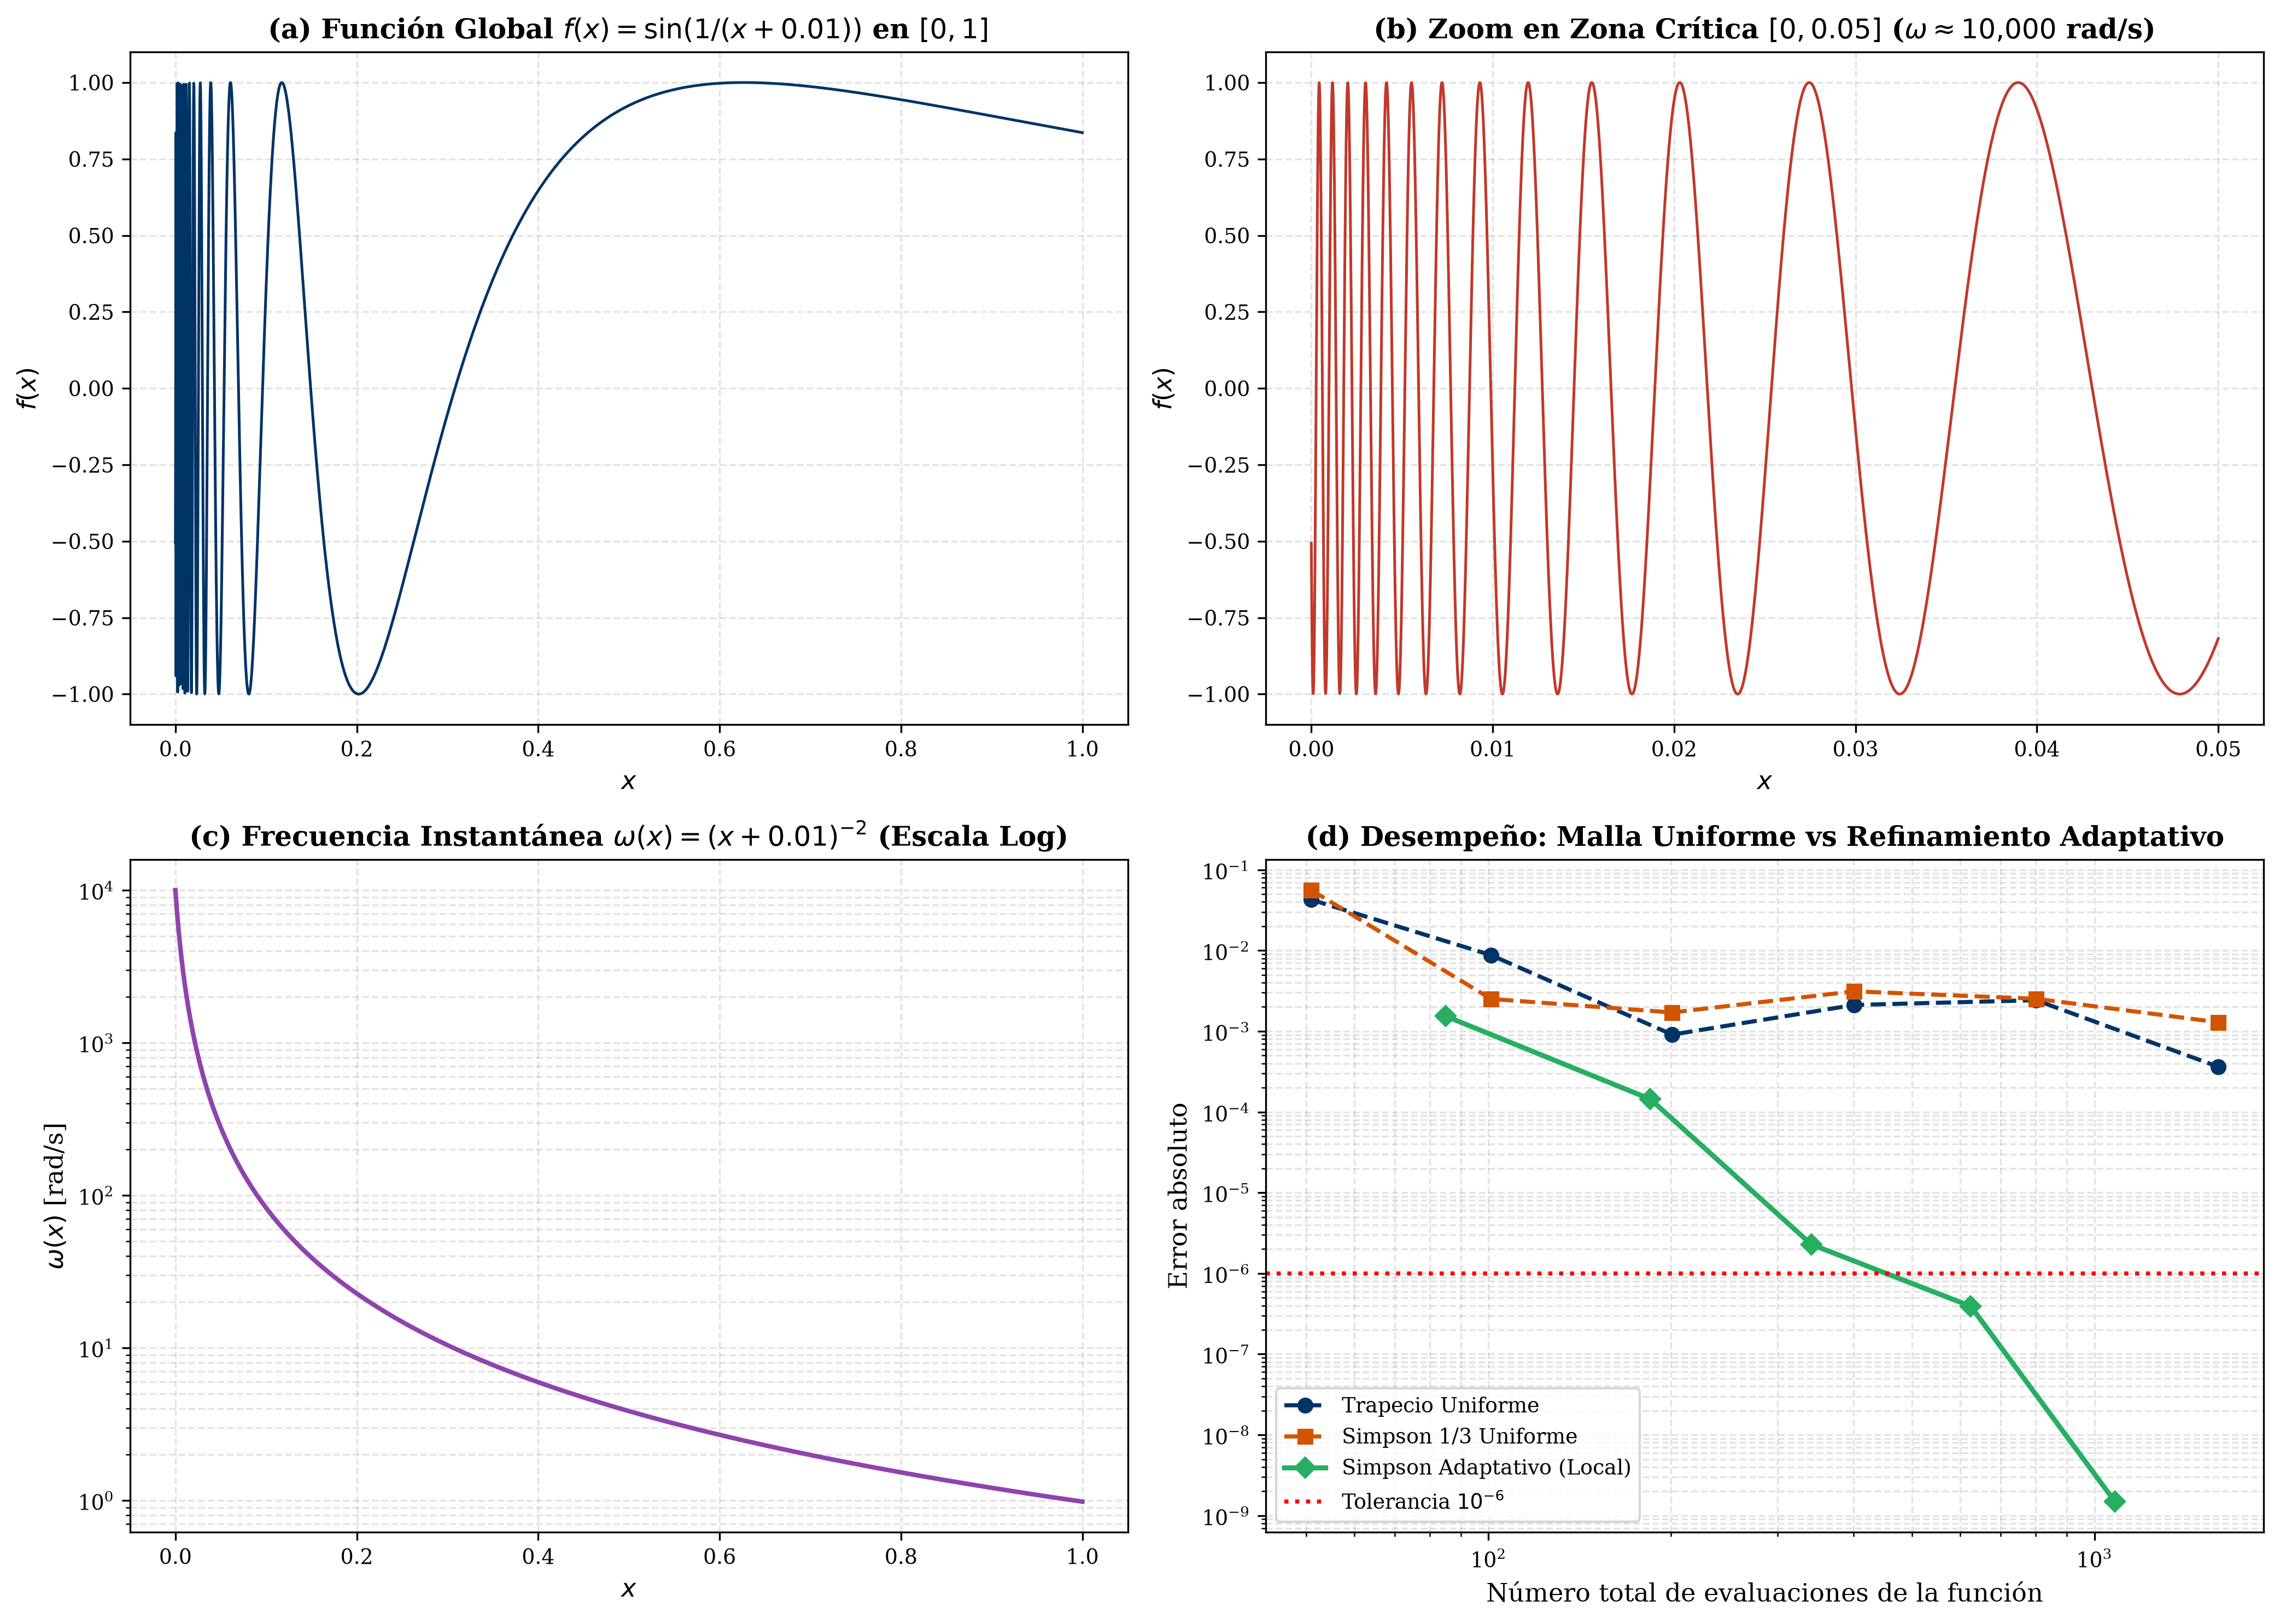
\includegraphics[width=0.98\textwidth]{fig_ejercicio6_altamente_oscilatoria.png}
    \caption{Ejercicio 6: (a) Señal completa en $[0, 1]$. (b) Acercamiento en zona de hiper-oscilación $[0, 0.05]$. (c) Frecuencia instantánea $\omega(x)$ en escala logarítmica. (d) Curvas de error vs. evaluaciones funcionales, evidenciando la superioridad radical del refinamiento adaptativo frente a la malla uniforme.}
    \label{fig:ejercicio6}
\end{figure}

% ==============================================================================
% SECCIÓN 8: CONCLUSIONES
% ==============================================================================
\section{Conclusiones Generales}

\begin{enumerate}[leftmargin=*]
    \item \textbf{Jerarquía de métodos sobre integrando suave:} Para polinomios y funciones suaves, los métodos de Newton-Cotes de segundo orden (Trapecio y Punto Medio) superan dramáticamente a las sumas de Riemann ($O(n^{-2})$ vs. $O(n^{-1})$). En la función exponencial, el trapecio requirió 1460 subintervalos para tolerancia $10^{-6}$, frente a los más de 6.38 millones necesarios por los rectángulos.
    \item \textbf{Efectos de simetría y cancelación de frontera:} En integrandos periódicos o con frontera nula como $\sin(x)$ en $[0, \pi]$, las sumas de Riemann coinciden con el trapecio y aceleran su convergencia natural a $O(n^{-2})$ debido a la cancelación del primer término impar en la expansión asintótica de Euler-Maclaurin.
    \item \textbf{Sensibilidad a la oscilación y aliasing:} Cuando el integrando presenta frecuencias espaciales elevadas, los métodos de cuadratura uniforme sufren de aliasing a menos que el paso $h$ cumpla la cota de Nyquist ($\omega_{\max} h < \pi$). En problemas con gradientes extremos de frecuencia, el refinamiento adaptativo local reduce el esfuerzo computacional en varios órdenes de magnitud al concentrar los nodos únicamente en las zonas de alta dinámica.
\end{enumerate}

\end{document}
